\chapter{Solutions of chapter 4\\
Cornerstone models: Conjugate families}\label{chap4}

\section{Solutions Exercises}\label{sec1}
\begin{enumerate}[leftmargin=*]
\item Write in the canonical form the distribution of the Bernoulli example, and find the mean and variance of the sufficient statistic.

\textbf{Answer}

Given $p({\bf{y}}|\theta)=(1-\theta)^N\exp\left\{\sum_{i=1}^N y_i\log\left(\frac{\theta}{1-\theta}\right)\right\}$ where $\eta=\log\frac{\theta}{1+\theta}$ which implies $\theta=\frac{\exp(\eta)}{1-\exp(\eta)}$, then $p({\bf{y}}|\theta)=\exp\left\{\sum_{i=1}^N y_i\eta-N\log(1+\exp(\eta))\right\}$. Thus $B(\eta)=N\log(1+\exp(\eta))$, $\nabla(B(\eta))=N\frac{\exp(\eta)}{1+\exp(\eta)}=N\theta$ and $\nabla^2(B(\eta))=N\left\{\frac{\exp(\eta)(1+\exp(\eta))}{(1+\exp(\eta))^2}-\frac{\exp(\eta)\exp(\eta)}{(1+\exp(\eta))^2}\right\}=N\theta(1-\theta)$. 



\item Given a random sample $\mathbf{y}=[y_1,y_2,\dots,y_N]^{\top}$ from $N$ \textit{binomial experiments} each having known size $n_i$ and same unknown probability $\theta$. Show that $p(\mathbf{y}|\theta)$ is in the exponential family, and find the posterior distribution, the marginal likelihood and the predictive distribution of the binomial-beta model assuming the number of trials is known.

\textbf{Answer}

The density function is 
\begin{align*}
p({\bf{y}}|\theta)&=\prod_{i=1}^N{n_i \choose y_i}\theta^{y_i}(1-\theta)^{n_i-y_i}\\
&=\prod_{i=1}^N{n_i \choose y_i}\theta^{\sum_{i=1}^Ny_i}(1-\theta)^{\sum_{i=1}^N n_i-\sum_{i=1}^N y_i}\\
&=\prod_{i=1}^N{n_i \choose y_i}\exp\left\{\sum_{i=1}^N y_i\log\left(\frac{\theta}{1-\theta}\right)+\sum_{i=1}^N n_i\log(1-\theta)\right\}\\
&=\prod_{i=1}^N{n_i \choose y_i}(1-\theta)^{\sum_{i=1}^N n_i}\exp\left\{\sum_{i=1}^N y_i\log\left(\frac{\theta}{1-\theta}\right)\right\},
\end{align*}
 
Observe that $\sum_{i=1}^N n_i$ is the total sample size of Bernoulli experiments. 

Using Theorem 1 in Chapter 4, the prior distribution is \begin{align*}\pi(\theta)&\propto(1-\theta)^{{\bf{B}}_0}\exp\left\{a_0\log\left(\frac{\theta}{1-\theta}\right)\right\}\\
	&=\theta^{a_0}(1-\theta)^{{\bf{B}}_0-a_0}\\
	&=\theta^{\alpha_0-1}(1-\theta)^{\beta_0-1},
\end{align*}

where $\alpha_0=a_0+1$ and $\beta_0={\bf{B}}_0-a_0+1$. This is the kernel of a beta distribution. Thus, the posterior distribution is

\begin{align*}
	\pi(\theta|{\bf{y}})&\propto \theta^{\alpha_0-1}(1-\theta)^{\beta_0-1} \times \theta^{\sum_{i=1}^Ny_i}(1-\theta)^{\sum_{i=1}^N n_i-\sum_{i=1}^N y_i}\\
	&=\theta^{\alpha_0+\sum_{i=1}^Ny_i - 1}(1-\theta)^{\beta_0 + \sum_{i=1}^N n_i-\sum_{i=1}^N y_i - 1}\\
	&=\theta^{\alpha_n-1}(1-\theta)^{\beta_n-1},  
\end{align*}

where $\alpha_n = \alpha_0+\sum_{i=1}^Ny_i$ and $\beta_n=\beta_0 + \sum_{i=1}^N n_i-\sum_{i=1}^N y_i$.

The marginal likelihood is

\begin{align*}
	p({\bf{y}})&=\int_0^1 \frac{\theta^{\alpha_0-1}(1-\theta)^{\beta_0-1}}{B(\alpha_0,\beta_0)}\times \prod_{i=1}^N{n_i \choose y_i}\theta^{\sum_{i=1}^Ny_i}(1-\theta)^{\sum_{i=1}^N n_i-\sum_{i=1}^N y_i} d\theta\\
	&=\frac{ \prod_{i=1}^N{n_i \choose y_i}}{B(\alpha_0,\beta_0)}\int_0^1 \theta^{\alpha_0+\sum_{i=1}^Ny_i-1}(1-\theta)^{}\beta_0\sum_{i=1}^N n_i-\sum_{i=1}^N y_i-1 d\theta\\
	&=\frac{ \prod_{i=1}^N{n_i \choose y_i}B(\alpha_n,\beta_n)}{B(\alpha_0,\beta_0)}. 
\end{align*}

The third line due to having the kernel of a Beta distribution.

Finally, the predictive distribution is

\begin{align*}
	p(Y_0|{\bf{y}})&=\int_0^1 {n_{y_0} \choose y_0} \theta^{y_0}(1-\theta)^{n_{y_0}-y_0}\frac{\theta^{\alpha_n-1}(1-\theta)^{\beta_n-1}}{B(\alpha_n,\beta_n)}d\theta\\
	&=\frac{{n_{y_0} \choose y_0}}{B(\alpha_n,\beta_n)}\int_0^1  \theta^{\alpha_n+y_0-1}(1-\theta)^{\beta_n+n_{y_0}-y_0-1}d\theta\\
	&={n_{y_0} \choose y_0}\frac{B(\alpha_n+y_0,\beta_n+n_{y_0}-y_0)}{B(\alpha_n,\beta_n)},
\end{align*}

where $n_{y_0}$ is the known size associated with $y_0$, and the last line due to having the kernel of a beta distribution. The predictive is a \textit{beta-binomial distribution}.

\item Given a random sample $\mathbf{y}=[y_1,y_2,\dots,y_N]^{\top}$ from a \textit{exponential distribution}. Show that $p(\mathbf{y}|\lambda)$ is in the exponential family, and find the posterior distribution, marginal likelihood and predictive distribution of the exponential-gamma model.

\textbf{Answer}

We see that the exponential distribution belongs to the exponential family as $p({\bf{y}}|\lambda)=\prod_{i=1}^N\lambda\exp(-\lambda y_i)=\lambda^N\exp(-\lambda\sum_{i=1}^N y_i)$.

Using the gamma distribution in the rate parametrization, we see that $\pi(\lambda|{\bf{y}})\propto \lambda^{\alpha_0-1}\exp(-\lambda\beta_0)\times \lambda^N\exp(-\lambda\sum_{i=1}^N y_i)=\lambda^{\alpha_0+N-1}\exp(-\lambda(\beta_0+\sum_{i=1}^N y_i))$. This is the kernel of a gamma distribution, that is, $\lambda|{\bf{y}}\sim G(\alpha_n,\beta_n)$ where $\alpha_n=\alpha_0+N$ and $\beta_n=\beta_0+\sum_{i=1}^N y_i$.

The marginal likelihood is

\begin{align*}
	p({\bf{y}})&=\int_0^{\infty}\lambda^N \exp\left\{-\lambda\sum_{i=1}^N\right\}\lambda^{\alpha_0-1}\exp\left\{-\beta_0\lambda\right\}\frac{\beta_0^{\alpha_0}}{\Gamma(\alpha_0)}d\lambda\\
	&=\frac{\beta_0^{\alpha_0}}{\Gamma(\alpha_0)}\int_0^{\infty}\lambda^{\alpha_0+N-1} \exp\left\{-\lambda\left(\beta_0+\sum_{i=1}^N\right)\right\}d\lambda\\
	&=\frac{\beta_0^{\alpha_0}\Gamma(\alpha_n)}{\Gamma(\alpha_0)\beta_n^{\alpha_n}}.
\end{align*} 

Finally, the predictive distribution is

\begin{align*}
	p(Y_0|{\bf{y}})&=\int_0^{\infty}\lambda \exp\left\{-\lambda y_0\right\}\lambda^{\alpha_n-1}\exp\left\{-\beta_n\lambda\right\}\frac{\beta_n^{\alpha_n}}{\Gamma(\alpha_n)}d\lambda\\
	&=\frac{\beta_n^{\alpha_n}}{\Gamma(\alpha_n)}\int_0^{\infty}\lambda^{\alpha_n+1-1}\exp\left\{-\lambda(\beta_n+y_0)\right\}d\lambda\\
	&=\frac{\beta_n^{\alpha_n}}{\Gamma(\alpha_n)}\times \frac{\Gamma(\alpha_n+1)}{(\beta_n+y_0)^{\alpha_n+1}}\\
	&=\frac{\alpha_n\beta_n^{\alpha_n}}{(\beta_n+y_0)^{\alpha_n+1}}.
\end{align*} 

This is a \textit{Lomax distribution}.

\item Given $\mathbf{y}\sim N_N(\mathbf{\mu},\mathbf{\mathbf{\mathbf{\Sigma}}})$, that is, a \textit{multivariate normal distribution} show that $p(\mathbf{y}|\mathbf{\mu},\mathbf{\mathbf{\mathbf{\Sigma}}})$ is in the exponential family.

\textbf{Answer} 

\begin{align}
	p(\mathbf{y}|\mathbf{\mu},\mathbf{\mathbf{\mathbf{\Sigma}}})&= (2\pi)^{-N/2}|\mathbf{\mathbf{\Sigma}}|^{-1/2}\exp\left\{-\frac{1}{2}\left(\mathbf{y}-\mathbf{\mu}\right)^{\top}\mathbf{\mathbf{\mathbf{\Sigma}}}^{-1}\left(\mathbf{y}-\mathbf{\mu}\right)\right\}\nonumber\\
	&= (2\pi)^{-N/2}\exp\left\{-\frac{1}{2}\left(\mathbf{y}^{\top}\mathbf{\mathbf{\Sigma}}^{-1}\mathbf{y}-2\mathbf{y}^{\top}\mathbf{\mathbf{\Sigma}}^{-1}\mathbf{\mu}+\mathbf{\mu}^{\top}\mathbf{\mathbf{\Sigma}}^{-1}\mathbf{\mu}+\log(|\mathbf{\Sigma}|)\right)\right\}\nonumber\\
	&= (2\pi)^{-N/2}\exp\left\{-\frac{1}{2}\left(tr\left\{\mathbf{y}^{\top}\mathbf{\mathbf{\Sigma}}^{-1}\mathbf{y}\right\}-2\mathbf{y}^{\top}\mathbf{\mathbf{\Sigma}}^{-1}\mathbf{\mu}+\mathbf{\mu}^{\top}\mathbf{\mathbf{\Sigma}}^{-1}\mathbf{\mu}+\log(|\mathbf{\Sigma}|)\right)\right\}\nonumber\\
	&= (2\pi)^{-N/2}\exp\left\{-\frac{1}{2}\left(vec\left(\mathbf{y}\mathbf{y}^{\top}\right)^{\top}vec\left(\mathbf{\mathbf{\Sigma}}^{-1}\right)-2\mathbf{y}^{\top}\mathbf{\mathbf{\Sigma}}^{-1}\mathbf{\mu}+\mathbf{\mu}^{\top}\mathbf{\mathbf{\Sigma}}^{-1}\mathbf{\mu}+\log(|\mathbf{\Sigma}|)\right)\right\} \nonumber, 	
\end{align}

where $tr$ and $vec$ are the trace and vectorization operators, respectively. 

Then, $h(\mathbf{y})=(2\pi)^{-N/2}$, $\eta(\mathbf{\mu},\mathbf{\mathbf{\Sigma}})=\left[\mathbf{\mathbf{\Sigma}}^{-1}\mathbf{\mu} \ \ vec\left(\mathbf{\mathbf{\Sigma}}^{-1}\right)\right]$, $T(\mathbf{y})=\left[\mathbf{y} \ \ -\frac{1}{2}vec(\mathbf{y}\mathbf{y}^{\top})\right]$ and $C(\mathbf{\mu},\mathbf{\mathbf{\Sigma}})=\exp\left\{-\frac{1}{2N}\left(\mathbf{\mu}^{\top}\mathbf{\mathbf{\Sigma}}^{-1}\mathbf{\mu}+\log(|\mathbf{\Sigma}|)\right)\right\}$.
	
\item Find the marginal likelihood in the normal/inverse-Wishart model.

\textbf{Answer}

\begin{align*}
	p({\bf{Y}})=&\int_{\mathcal{R}^p}\int_{\mathcal{S}}(2\pi)^{-pN/2}|\mathbf{\Sigma}|^{-N/2}\exp\left\{-\frac{1}{2}tr[({\bf{S}}+N(\mu-\hat{\mu})(\mu-\hat{\mu})^{\top})\mathbf{\Sigma}^{-1}]\right\}\\
	&\times (2\pi)^{-p/2}\beta_0^{p/2}|\mathbf{\Sigma}|^{-1/2}\exp\left\{-\frac{\beta_0}{2}tr[(\mu-\mu_0)(\mu-\mu_0)^{\top}\mathbf{\Sigma}^{-1}]\right\}\\
	&\times |\mathbf{\Sigma}|^{-(\alpha_0+p+1)/2}\frac{2^{-\alpha_0p/2}|\mathbf{\Psi}_0|^{\alpha_0/2}}{\Gamma_p(\alpha_0/2)}\exp\left\{-\frac{1}{2}tr(\mathbf{\Psi}_0\mathbf{\Sigma}^{-1})\right\}d\mathbf{\Sigma} d\mu\\
	&=\frac{(2\pi)^{-frac{1}{2}(pN+p)}|\mathbf{\Psi}_0|^{\alpha_0/2}\beta_0^{p/2}2^{-\alpha_0p/2}}{\Gamma_p(\alpha_0/2)}\int_{\mathcal{R}^p}\int_{\mathcal{S}} |\mathbf{\Sigma}|^{-\frac{1}{2}(N+1+\alpha_0+p+1)}\\
	&\times \exp\left\{-\frac{1}{2}tr[({\bf{S}}+N(\mu-\hat{\mu})(\mu-\hat{\mu})^{\top}+\beta_0(\mu-\mu_0)(\mu-\mu_0)^{\top}+\mathbf{\Psi}_0)\mathbf{\Sigma}^{-1}]\right\}d\mathbf{\Sigma} d\mu.
\end{align*}

We have in the integral the kernel of an Inverse-Wishart distribution, then

\begin{align*}
p({\bf{Y}})	&=\frac{\Gamma_p\left(\frac{N+1+\alpha_0}{2}\right)|\mathbf{\Psi}_0|^{\alpha_0/2}\beta_0^{p/2}}{\Gamma_p(\alpha_0/2)\pi^{p(N+1)/2}}\\
	&\times\int_{\mathcal{R}^p} |{\bf{S}}+\mathbf{\Psi}_0+(N+\beta_0)(\mu-\mu_n)(\mu-\mu_n)^{\top}\\
	&+N\beta_0/(N+\beta_0)(\hat{\mu}-\mu_0)(\hat{\mu}-\mu_0)^{\top}| d\mu\\
	&=\frac{\Gamma_p\left(\frac{N+1+\alpha_0}{2}\right)|\mathbf{\Psi}_0|^{\alpha_0/2}\beta_0^{p/2}}{\Gamma_p(\alpha_0/2)\pi^{p(N+1)/2}}\\
	&\times\int_{\mathcal{R}^p} |\mathbf{\Psi}_n||1+\beta_n(\mu-\mu_n)\mathbf{\Psi}_n^{-1}(\mu-\mu_n)^{\top}|^{-\frac{1}{2}(\alpha_n+1)} d\mu\\
	&=\frac{\Gamma_p\left(\frac{\alpha_n+1}{2}\right)|\mathbf{\Psi}_0|^{\alpha_0/2}\beta_0^{p/2}}{\Gamma_p(\alpha_0/2)\pi^{p(N+1)/2}}|\mathbf{\Psi}_n|^{-\frac{1}{2}(\alpha_n+1)}\\
	&\times\int_{\mathcal{R}^p} [1+\beta_n(\mu-\mu_n)^{\top}\mathbf{\Psi}_n^{-1}(\mu-\mu_n)]^{-\frac{1}{2}(\alpha_n+1)} d\mu.
\end{align*} 

The last equality uses the definition of $\mathbf{\Psi}_n$, $\beta_n$ and $\alpha_n$, and the Sylvester's determinant theorem. Observe that we have the kernel of a multivariate t distribution \cite{murphy2007conjugate}. Then,

\begin{align*}
	p({\bf{Y}})	&=\frac{\Gamma_p\left(\frac{\alpha_n+1}{2}\right)|\mathbf{\Psi}_0|^{\alpha_0/2}\beta_0^{p/2}}{\Gamma_p(\alpha_0/2)\pi^{p(N+1)/2}}|\mathbf{\Psi}_n|^{-\frac{1}{2}(\alpha_n+1)}\\
	&\times\int_{\mathcal{R}^p} \left[ 1+\frac{1}{\alpha_n+1-p}(\mu-\mu_n)^{\top}\left(\frac{\mathbf{\Psi}_n}{\beta_n(\alpha_n+1-p)}\right)^{-1}(\mu-\mu_n)\right]^{-\frac{1}{2}(\alpha_n+1-p+p)} d\mu\\
	&=\frac{\Gamma_p\left(\frac{\alpha_n+1}{2}\right)\Gamma_p\left(\frac{\alpha_n+1-p}{2}\right)|\mathbf{\Psi}_0|^{\alpha_0/2}\beta_0^{p/2}(\alpha_n+1-p)^{p/2}\pi^{p/2}|\mathbf{\Psi}_n|^{-\frac{1}{2}(\alpha_n+1)}}{\Gamma_p(\alpha_0/2)\pi^{p(N+1)/2}\Gamma_p\left(\frac{\alpha_n+1-p+p}{2}\right)\left(\frac{\mathbf{\Psi}_n}{\alpha_n+1-p}\right)^{-1/2}}\\
	&=\frac{\Gamma_p\left(\frac{v_n}{2}\right)}{\Gamma_p\left(\frac{\alpha_0}{2}\right)}\frac{|\mathbf{\Psi}_0|^{\alpha_0/2}}{|\mathbf{\Psi}_n|^{\alpha_n/2}}\left(\frac{\beta_0}{\beta_n}\right)^{p/2}(2\pi)^{-Np/2},
\end{align*}

where $v_n=\alpha_n+1-p$.


\item Find the posterior predictive distribution in the normal/inverse-Wishart model, and show that ${\bf{Y}}_0|{\bf{Y}}\sim T_{N_0,M}(\alpha_n-M+1,{\bf{X}}_0{\bf{B}}_n,{\bf{I}}_{N_0}+{\bf{X}}_0{\bf{V}}_n{\bf{X}}_0^{\top},{\bf{\Psi}}_n)$ in the multivariate regression linear model.

\textbf{Answer}

\begin{align*}
	p({\bf{Y}}_0|{\bf{Y}})&\propto\int_{\mathcal{R}^p}\int_{\mathcal{S}}|\mathbf{\Sigma}|^{-1/2}\exp\left\{-\frac{1}{2}tr[({\bf{y}}_0-\mu)({\bf{y}}_0-\mu)^{\top}\mathbf{\Sigma}^{-1}]\right\}\\
	&\times |\mathbf{\Sigma}|^{-1/2}\exp\left\{-\frac{\beta_n}{2}tr[(\mu-\mu_n)(\mu-\mu_n)^{\top}\mathbf{\Sigma}^{-1}]\right\}\\
	&\times |\mathbf{\Sigma}|^{-(\alpha_n+p+1)/2}\exp\left\{-\frac{1}{2}tr(\mathbf{\Psi}_n \mathbf{\Sigma}^{-1})\right\}d\mathbf{\Sigma} d\mu\\
	&\propto\int_{\mathcal{R}^p}|({\bf{y}}_0-\mu)({\bf{y}}_0-\mu)^{\top}+(\mu-\mu_n)(\mu-\mu_n)^{\top}+\mathbf{\Psi}_n|^{-(\alpha_n+2)/2}d\mu.
\end{align*}

The last equality uses that there is the kernel of an Inverse Wishart distribution.

Taking into account that

{\scriptsize{
\begin{align*}
	({\bf{y}}_0-\mu)({\bf{y}}_0-\mu)^{\top}+(\mu-\mu_n)(\mu-\mu_n)^{\top} & = (1+\beta_n)\left(\mu-\frac{({\bf{y}}_0+\beta_n\mu_n)}{1+\beta_n}\right)\left(\mu-\frac{({\bf{y}}_0+\beta_n\mu_n)}{1+\beta_n}\right)^{\top}\\
	&+\frac{\beta_n}{1+\beta_n}({\bf{y}}_0-\mu_n)({\bf{y}}_0-\mu_n)^{\top}.
\end{align*}
}}

Then,
{\scriptsize{
\begin{align*}
	p({\bf{Y}}_0|{\bf{Y}})&\propto\int_{\mathcal{R}^p}|({\bf{y}}_0-\mu)({\bf{y}}_0-\mu)^{\top}+(\mu-\mu_n)(\mu-\mu_n)^{\top}+\mathbf{\Psi}_n|^{-(\alpha_n+2)/2}d\mu\\
	&=\int_{\mathcal{R}^p}\left\vert(1+\beta_n)\left(\mu-\frac{({\bf{y}}_0+\beta_n\mu_n)}{1+\beta_n}\right)\left(\mu-\frac{({\bf{y}}_0+\beta_n\mu_n)}{1+\beta_n}\right)^{\top}\right.\\
	&\left.+\frac{\beta_n}{1+\beta_n}({\bf{y}}_0-\mu_n)({\bf{y}}_0-\mu_n)^{\top}+\mathbf{\Psi}_n\right\vert^{-(\alpha_n+2)/2}d\mu\\
	&=\int_{\mathcal{R}^p}\left[\left\vert\underbrace{\mathbf{\Psi}_n+\frac{\beta_n}{1+\beta_n}({\bf{y}}_0-\mu_n)({\bf{y}}_0-\mu_n)^{\top}}_{\mathbf{\Lambda}_n}\right\vert\right.\\
	&\left.\left\vert 1+(1+\beta_n)\left(\mu-\frac{({\bf{y}}_0+\beta_n\mu_n)}{1+\beta_n}\right)^{\top}\frac{1}{\alpha_n+2-p}\left(\frac{\mathbf{\Lambda}_n}{\alpha_n+2-p}\right)^{-1}\left(\mu-\frac{({\bf{y}}_0+\beta_n\mu_n)}{1+\beta_n}\right)\right\vert\right]^{-(\alpha_n+2-p+p)/2}d\mu\\
	&\propto \left\vert\mathbf{\Psi}_n+\frac{\beta_n}{1+\beta_n}({\bf{y}}_0-\mu_n)({\bf{y}}_0-\mu_n)^{\top}\right\vert^{-(\alpha_n+2)/2}\\
	&\times \left\vert\mathbf{\Psi}_n+\frac{\beta_n}{1+\beta_n}({\bf{y}}_0-\mu_n)({\bf{y}}_0-\mu_n)^{\top}\right\vert^{1/2}\\
	&=\left\vert\mathbf{\Psi}_n+\frac{\beta_n}{1+\beta_n}({\bf{y}}_0-\mu_n)({\bf{y}}_0-\mu_n)^{\top}\right\vert^{-(\alpha_n+1)/2}\\
	&\propto \left[1+({\bf{y}}_0-\mu_n)^{\top}\frac{1}{\alpha_n+1-p}\left(\frac{\mathbf{\Psi}_n(1+\beta_n)}{(\alpha_n+1-p)\beta_n}\right)^{-1}({\bf{y}}_0-\mu_n)\right]^{-(\alpha_n+1-p+p)}. 
\end{align*} 
}}

The second equality and last line use the Sylvester's determinant theorem, and the second equality uses that there is the kernel of a multivariate t distribution.

Then, we have that the predictive distribution is a multivariate t distribution centered at $\mu_n$, $\alpha_n+1-p$ degrees of freedom, and scale matrix $\frac{\mathbf{\Psi}_n(1+\beta_n)}{(\alpha_n+1-p)\beta_n}$.

To show the second statement, let's start by the definition of the predictive density to show that ${\bf{Y}}_0|{\bf{Y}}\sim T_{N_0,M}(\alpha_n-M+1,{\bf{X}}_0{\bf{B}}_n,{\bf{I}}_{N_0}+{\bf{X}}_0{\bf{V}}_n{\bf{X}}_0^{\top},{\bf{\Psi}}_n)$.

\begin{align*}
	\pi({\bf{Y}}_0|{\bf{Y}})&\propto\int_{\mathcal{S}}\int_{\mathcal{B}}\left\{ |{\bf{\Sigma}}|^{-N_0/2}\exp\left\{-\frac{1}{2}tr[({\bf{Y}}_0-{\bf{X}}_0{\bf{B}})^{\top}({\bf{Y}}_0-{\bf{X}}_0{\bf{B}}){\bf{\Sigma}^{-1}}]\right\}\right.\\
	&\times |{\bf{\Sigma}}|^{-K/2}\exp\left\{-\frac{1}{2}tr[({\bf{B}}-{\bf{B}}_n)^{\top}{\bf{V}}_n^{-1}({\bf{B}}-{\bf{B}}_n){\bf{\Sigma}^{-1}}]\right\}\\
	&\times\left. |{\bf{\Sigma}}|^{-(\alpha_n+M+1)/2}\exp\left\{-\frac{1}{2}tr[{\bf{\Psi}}_n{\bf{\Sigma}^{-1}}]\right\}\right\}d{\bf{B}}d{\bf{\Sigma}}\\
	&=\int_{\mathcal{S}}\int_{\mathcal{B}}\left\{ |{\bf{\Sigma}}|^{-(N_0+K+\alpha_n+M+1)/2}\exp\left\{-\frac{1}{2}tr\left[\left(({\bf{Y}}_0-{\bf{X}}_0{\bf{B}})^{\top}({\bf{Y}}_0-{\bf{X}}_0{\bf{B}})\right.\right.\right.\right.\\
	&\left.\left.\left.\left.+({\bf{B}}-{\bf{B}}_n)^{\top}{\bf{V}}_n^{-1}({\bf{B}}-{\bf{B}}_n)+{\bf{\Psi}}_n\right){\bf{\Sigma}^{-1}}\right]\right\}\right\}d{\bf{B}}d{\bf{\Sigma}}.	 
\end{align*}

Setting ${\bf{M}}=({\bf{X}}_0^{\top}{\bf{X}}_0+{\bf{V}}_n^{-1})$, and ${\bf{B}}_{*}={\bf{M}}^{-1}({\bf{V}}_n{\bf{B}}_n+{\bf{X}}_0^{\top}{\bf{Y}}_0)$, we have that $({\bf{B}}-{\bf{B}}_*)^{\top}{\bf{M}}({\bf{B}}-{\bf{B}}_*)+{\bf{B}}_n^{\top}{\bf{V}}_n^{-1}{\bf{B}}_n+{\bf{Y}}_0^{\top}{\bf{Y}}_0-{\bf{B}}_*^{\top}{\bf{M}}{\bf{B}}_*=({\bf{Y}}_0-{\bf{X}}_0{\bf{B}})^{\top}({\bf{Y}}_0-{\bf{X}}_0{\bf{B}})+({\bf{B}}-{\bf{B}}_n)^{\top}{\bf{V}}_n^{-1}({\bf{B}}-{\bf{B}}_n)$. Then,

\begin{align*}
	\pi({\bf{Y}}_0|{\bf{Y}})&\propto \int_{\mathcal{S}}|{\bf{\Sigma}}|^{-(N_0+K+\alpha_n+M+1)/2}\\
	&\times \exp\left\{-\frac{1}{2}tr[({\bf{\Psi}}_n+{\bf{B}}_n^{\top}{\bf{V}}_n^{-1}{\bf{B}}_n+{\bf{Y}}_0^{\top}{\bf{Y}}_0-{\bf{B}}_*^{\top}{\bf{M}}{\bf{B}}_*){\bf{\Sigma}^{-1}}]\right\}\\
	&\times\int_{\mathcal{B}}\exp\left\{-\frac{1}{2}tr[({\bf{B}}-{\bf{B}}_*)^{\top}{\bf{M}}({\bf{B}}-{\bf{B}}_*){\bf{\Sigma}^{-1}}]\right\}d{\bf{B}}d{\bf{\Sigma}}.
\end{align*} 

The latter is the kernel of a matrix normal distribution, thus

\begin{align*}
	\pi({\bf{Y}}_0|{\bf{Y}})&\propto \int_{\mathcal{S}}|{\bf{\Sigma}}|^{-(N_0+\alpha_n+M+1)/2}\\
	&\times \exp\left\{-\frac{1}{2}tr[({\bf{\Psi}}_n+{\bf{B}}_n^{\top}{\bf{V}}_n^{-1}{\bf{B}}_n+{\bf{Y}}_0^{\top}{\bf{Y}}_0-{\bf{B}}_*^{\top}{\bf{M}}{\bf{B}}_*){\bf{\Sigma}^{-1}}]\right\}d{\bf{\Sigma}}\\
\end{align*}

This is the kernel of an inverse-Wishart distribution, then

\begin{align*}
	\pi({\bf{Y}}_0|{\bf{Y}})&\propto \left|{\bf{\Psi}}_n+{\bf{B}}_n^{\top}{\bf{V}}_n^{-1}{\bf{B}}_n+{\bf{Y}}_0^{\top}{\bf{Y}}_0-{\bf{B}}_*^{\top}{\bf{M}}{\bf{B}}_*\right|^{-(N_0+\alpha_n)/2}.
\end{align*} 

Setting ${\bf{C}}^{-1}={\bf{I}}_{N_0}+{\bf{X}}_0{\bf{V}}_n{\bf{X}}_0^{\top}$ such that ${\bf{C}}={\bf{I}}_{N_0}-{\bf{X}}_0({\bf{X}}_0^{\top}{\bf{X}}_0+{\bf{V}}_n^{-1})^{-1}{\bf{X}}_0^{\top}$ (see footnote 4 in Chapter 4), then ${\bf{B}}_n^{\top}{\bf{V}}_n^{-1}{\bf{B}}_n+{\bf{Y}}_0^{\top}{\bf{Y}}_0-{\bf{B}}_*^{\top}{\bf{M}}{\bf{B}}_*=({\bf{Y}}_0-{\bf{X}}_0{\bf{B}}_n)^{\top}{\bf{C}}({\bf{Y}}_0-{\bf{X}}_0{\bf{B}}_n)$. This is done following exactly same procedure as deducing the predictive distribution in the linear regression model in the book. Thus,
\begin{align*}
	\pi({\bf{Y}}_0|{\bf{Y}})&\propto \left|{\bf{\Psi}}_n+({\bf{Y}}_0-{\bf{X}}_0{\bf{B}}_n)^{\top}{\bf{C}}({\bf{Y}}_0-{\bf{X}}_0{\bf{B}}_n)\right|^{-(N_0+\alpha_n)/2}\\
	&\propto\left|{\bf{I}}_{N_0}+{\bf{C}}({\bf{Y}}_0-{\bf{X}}_0{\bf{B}}_n){\bf{\Psi}}^{-1}({\bf{Y}}_0-{\bf{X}}_0{\bf{B}}_n)^{\top}\right|^{-(\alpha_n+1-M+N_0+M-1)/2}.
\end{align*} 
The second proportionality follows from the Sylvester's theorem. Observe that this is the kernel of a matrix t distribution with $\alpha_n+1-M$ degrees of freedom, location ${\bf{X}}_0{\bf{B}}_n$ and scale matrices ${\bf{\Psi}}_n$ and ${\bf{C}}^{-1}={\bf{I}}_{N_0}+{\bf{X}}_0{\bf{V}}_n{\bf{X}}_0^{\top}$.     

\item Show that $\delta_n=\delta_0+({\bf{y}}-{\bf{X}}\hat{\beta})^{\top}({\bf{y}}-{\bf{X}}\hat{\beta})+(\hat{\beta}-\beta_0)^{\top}(({\bf{X}}^{\top}{\bf{X}})^{-1}+{\bf{B}}_0)^{-1}(\hat{\beta}-\beta_0)$ in the linear regression model, and that ${\bf{\Psi}}_{n}={\bf{\Psi}}_{0}+{\bf{S}}+(\hat{\bf{B}}-{\bf{B}}_{0})^{\top}{\bf{V}}_{n}(\hat{\bf{B}}-{\bf{B}}_{0})$ in the linear multivariate regression model. 

\textbf{Answer}

Taking into account that 
\begin{align*}
	\delta^* & = \delta_0 + {\bf{y}}^{\top}{\bf{y}} + \beta_0^{\top}{\bf{B}}_0^{-1}\beta_0 - \beta_n^{\top}{\bf{B}}_n^{-1}\beta_n \\
	& = \delta_0 + {\bf{y}}^{\top}{\bf{y}} + \beta_0^{\top}{\bf{B}}_0^{-1}\beta_0 -({\bf{B}}_0^{-1}\beta_0 + {\bf{X}}^{\top}{\bf{X}}\hat{\beta})^{\top}{\bf{B}}_n({\bf{B}}_0^{-1}\beta_0 + {\bf{X}}^{\top}{\bf{X}}\hat{\beta}) \\
	& = \delta_0 + {\bf{y}}^{\top}{\bf{y}} - \hat{\beta}^{\top}{\bf{X}}^{\top}{\bf{X}}{\bf{B}}_n{\bf{X}}^{\top}{\bf{X}}\hat{\beta} - 2\hat{\beta}^{\top}{\bf{X}}^{\top}{\bf{X}}{\bf{B}}_n{\bf{B}}_0^{-1}\beta_0 + \beta_0^{\top}({\bf{B}}_0^{-1} - {\bf{B}}_0^{-1}{\bf{B}}_n{\bf{B}}_0^{-1})\beta_0 \\
	&- \hat{\beta}^{\top}{\bf{X}}^{\top}{\bf{X}}\hat{\beta} + \hat{\beta}^{\top}{\bf{X}}^{\top}{\bf{X}}\hat{\beta} \\
	& = \delta_0 + {\bf{y}}^{\top}{\bf{y}} - \hat{\beta}^{\top}{\bf{X}}^{\top}{\bf{X}}\hat{\beta} + \hat{\beta}^{\top}({\bf{X}}^{\top}{\bf{X}} - {\bf{X}}^{\top}{\bf{X}}{\bf{B}}_n{\bf{X}}^{\top}{\bf{X}})\hat{\beta} \\
	& - 2\hat{\beta}^{\top}{\bf{X}}^{\top}{\bf{X}}{\bf{B}}_n{\bf{B}}_0^{-1}\beta_0 + \beta_0^{\top}({\bf{B}}_0^{-1} - {\bf{B}}_0^{-1}{\bf{B}}_n{\bf{B}}_0^{-1})\beta_0. 
\end{align*}

Observe that 
\begin{align*}
	({\bf{y}} - {\bf{X}}\hat{\beta})^{\top}({\bf{y}} - {\bf{X}}\hat{\beta}) & = {\bf{y}}^{\top}{\bf{y}} - 2\hat{\beta}{\bf{X}}^{\top}{\bf{y}} + \hat{\beta}^{\top}{\bf{X}}^{\top}{\bf{X}}\hat{\beta}\\
	& = {\bf{y}}^{\top}{\bf{y}} - 2\hat{\beta}^{\top}{\bf{X}}^{\top}({\bf{X}}\hat{\beta}+\hat{\mu}) + \hat{\beta}^{\top}{\bf{X}}^{\top}{\bf{X}}\hat{\beta}\\
	& = {\bf{y}}^{\top}{\bf{y}} - \hat{\beta}^{\top}{\bf{X}}^{\top}{\bf{X}}\hat{\beta},
\end{align*}
where ${\bf{y}}={\bf{X}}\hat{\beta}+\hat{\mu}$, and ${\bf{X}}^{\top}\hat{\mu}=0$.

The following matrix identities are useful \cite{Smith1973}:
%\begin{equation}\label{eq:a}
%D + E & = E(E^{-1} + D^{-1})D
%\end{equation}

\begin{equation*}
	({\bf{D}} + {\bf{E}})^{-1} = {\bf{D}}^{-1} - {\bf{D}}^{-1}({\bf{D}}^{-1} + {\bf{E}}^{-1})^{-1}{\bf{D}}^{-1},
\end{equation*}
and
\begin{equation*}
	({\bf{D}} + {\bf{E}})^{-1} = {\bf{D}}^{-1}({\bf{E}}^{-1} + {\bf{D}}^{-1}){\bf{E}}^{-1}.
\end{equation*}

Using these identities,
\begin{align*}
	[({\bf{X}}^{\top}{\bf{X}})^{-1} + {\bf{B}}_0]^{-1} & = {\bf{X}}^{\top}{\bf{X}} - {\bf{X}}^{\top}{\bf{X}}({\bf{X}}^{\top}{\bf{X}} + {\bf{B}}_0^{-1})^{-1}{\bf{X}}^{\top}{\bf{X}} \\
	& = {\bf{B}}_0^{-1} - {\bf{B}}_0^{-1}({\bf{X}}^{\top}{\bf{X}} + {\bf{B}}_0^{-1})^{-1}{\bf{B}}_0^{-1}\\
	& = {\bf{X}}^{\top}{\bf{X}}({\bf{X}}^{\top}{\bf{X}} + {\bf{B}}_0^{-1})^{-1}{\bf{B}}_0^{-1}. 
\end{align*}
Then, 
\begin{align*}
	\delta^* & = \delta_0+ ({\bf{y}} - {\bf{X}}\hat{\beta})^{\top}({\bf{y}} - {\bf{X}}\hat{\beta}) + \hat{\beta}^{\top}[({\bf{X}}^{\top}{\bf{X}})^{-1} + {\bf{B}}_0]^{-1}\hat{\beta} \\
	& - 2\hat{\beta}[({\bf{X}}^{\top}{\bf{X}})^{-1} + {\bf{B}}_0]^{-1}\beta_0 + \beta_0^{\top}[({\bf{X}}^{\top}{\bf{X}})^{-1} + {\bf{B}}_0]^{-1}\beta_0\\
	& = \delta_0+ ({\bf{y}} - {\bf{X}}\hat{\beta})^{\top}({\bf{y}} - {\bf{X}}\hat{\beta})\\
	& + (\hat{\beta} - \beta_0)^{\top}[({\bf{X}}^{\top}{\bf{X}})^{-1} + {\bf{B}}_0]^{-1}(\hat{\beta} - \beta_0).
\end{align*}

In a similar way for the second part,

\begin{align*}
	({\bf{V}}_0+({\bf{X}}^{\top}{\bf{X}})^{-1})^{-1}&={\bf{V}}_0^{-1}-{\bf{V}}_0^{-1}({\bf{V}}_0^{-1}+{\bf{X}}^{\top}{\bf{X}})^{-1}{\bf{V}}_0^{-1}\\
	&={\bf{X}}^{\top}{\bf{X}}-{\bf{X}}^{\top}{\bf{X}}({\bf{V}}_0^{-1}+{\bf{X}}^{\top}{\bf{X}})^{-1}{\bf{X}}^{\top}{\bf{X}}\\
	&={\bf{X}}^{\top}{\bf{X}}(({\bf{X}}^{\top}{\bf{X}})^{-1}+{\bf{V}}_0)^{-1}{\bf{V}}_0^{-1},
\end{align*}

we use these results and some algebra to show that ${\bf{B}}_{0}^{\top}{\bf{V}}_{0}^{-1}{\bf{B}}_{0}+\widehat{\bf{B}}^{\top}{\bf{X}}^{\top}{\bf{X}}\widehat{\bf{B}}-{\bf{B}}_n^{\top}{\bf{V}}_n^{-1}{\bf{B}}_n=(\hat{\bf{B}}-{\bf{B}}_{0})^{\top}{\bf{V}}_{n}(\hat{\bf{B}}-{\bf{B}}_{0})$ taking into account that ${\bf{V}}_n = ({\bf{V}}_{0}^{-1}+{\bf{X}}^{\top}{\bf{X}})^{-1}$ and $\widehat{\bf{B}}= ({\bf{X}}^{\top}{\bf{X}})^{-1}{\bf{X}}^{\top}{\bf{Y}}$.


\item Show that in the linear regression model $\beta_n^{\top}({\bf{B}}_n^{-1}-{\bf{B}}_n^{-1}{\bf{M}}^{-1}{\bf{B}}_n^{-1})\beta_n={\bf{\beta}}_{**}^{\top}{\bf{C}}{\bf{\beta}}_{**}$ and $\beta_{**}={\mathbf{X}}_0\beta_n$.

\textbf{Answer}

Taking into account that $({\bf{A}}+{\bf{B}})^{-1}={\bf{A}}^{-1}-{\bf{A}}^{-1}({\bf{A}}^{-1}+{\bf{B}}^{-1})^{-1}{\bf{A}}^{-1}$ \cite{Smith1973}, then we observe that $({\bf{B}}_n^{-1}-{\bf{B}}_n^{-1}{\bf{M}}^{-1}{\bf{B}}_n^{-1})=({\bf{B}}_n+({\bf{X}}_0^{\top}{\bf{X}}_0)^{-1})^{-1}$, where $({\bf{B}}_n+({\bf{X}}_0^{\top}{\bf{X}}_0)^{-1})^{-1}={\bf{X}}_0^{\top}{\bf{X}}_0-{\bf{X}}_0^{\top}{\bf{X}}_0({\bf{B}}_n^{-1}+{\bf{X}}_0^{\top}{\bf{X}}_0)^{-1}{\bf{X}}_0^{\top}{\bf{X}}_0={\bf{X}}_0^{\top}{\bf{X}}_0-{\bf{X}}_0^{\top}{\bf{X}}_0{\bf{M}}^{-1}{\bf{X}}_0^{\top}{\bf{X}}_0$, thus
\begin{align*}
	\beta_n^{\top}({\bf{B}}_n^{-1}-{\bf{B}}_n^{-1}{\bf{M}}^{-1}{\bf{B}}_n^{-1})\beta_n&=\beta_n^{\top}({\bf{X}}_0^{\top}{\bf{X}}_0-{\bf{X}}_0^{\top}{\bf{X}}_0{\bf{M}}^{-1}{\bf{X}}_0^{\top}{\bf{X}}_0)\beta_n\\
	&=\beta_n^{\top}{\bf{X}}_0^{\top}({\bf{I}}_{N_0}-{\bf{X}}_0{\bf{M}}^{-1}{\bf{X}}_0^{\top}){\bf{X}}_0\beta_n\\
	&=\beta_n^{\top}{\bf{X}}_0^{\top}{\bf{C}}{\bf{X}}_0\beta_n\\
	&={\bf{\beta}}_{**}^{\top}{\bf{C}}{\bf{\beta}}_{**}.
\end{align*}

Let's show that $\beta_{**}={\mathbf{X}}_0\beta_n$,

\begin{align*}
	\beta_{**}&={\bf{C}}^{-1}{\bf{X}}_0{\bf{M}}^{-1}{\bf{B}}_n^{-1}\beta_n\\
	&=({\bf{I}}_{N_0}+{\bf{X}}_0{\bf{B}}_n{\bf{X}}_0^{\top}){\bf{X}}_0{\bf{M}}^{-1}{\bf{B}}_n^{-1}\beta_n\\
	&=({\bf{I}}_{N_0}+{\bf{X}}_0{\bf{B}}_n{\bf{X}}_0^{\top}){\bf{X}}_0({\bf{B}}_n-{\bf{B}}_n(({\bf{X}}_0^{\top}{\bf{X}}_0)^{-1}+{\bf{B}}_n)^{-1}{\bf{B}}_n){\bf{B}}_n^{-1}\beta_n\\
	&=({\bf{I}}_{N_0}+{\bf{X}}_0{\bf{B}}_n{\bf{X}}_0^{\top})({\bf{X}}_0\beta_n-{\bf{X}}_0{\bf{B}}_n(({\bf{X}}_0^{\top}{\bf{X}}_0)^{-1}+{\bf{B}}_n)^{-1}\beta_n)\\
	&={\bf{X}}_0\beta_n-{\bf{X}}_0{\bf{B}}_n(({\bf{X}}_0^{\top}{\bf{X}}_0)^{-1}+{\bf{B}}_n)^{-1}\beta_n+{\bf{X}}_0{\bf{B}}_n{\bf{X}}_0^{\top}{\bf{X}}_0\beta_n\\
	&-{\bf{X}}_0{\bf{B}}_n{\bf{X}}_0^{\top}{\bf{X}}_0{\bf{B}}_n(({\bf{X}}_0^{\top}{\bf{X}}_0)^{-1}+{\bf{B}}_n)^{-1}\beta_n\\
	&={\bf{X}}_0\beta_n-{\bf{X}}_0{\bf{B}}_n[(({\bf{X}}_0^{\top}{\bf{X}}_0)^{-1}+{\bf{B}}_n)^{-1}-{\bf{X}}_0^{\top}{\bf{X}}_0+{\bf{X}}_0^{\top}{\bf{X}}_0{\bf{B}}_n(({\bf{X}}_0^{\top}{\bf{X}}_0)^{-1}+{\bf{B}}_n)^{-1}]\beta_n.
\end{align*}

Using that $({\bf{A}}+{\bf{B}})^{-1}={\bf{A}}^{-1}-{\bf{A}}^{-1}{\bf{B}}({\bf{A}}+{\bf{B}})^{-1}$, we observe that the expression in brackets is equal to ${\bf{0}}$, then we have the result.

\item Show that $({\bf{Y}}-{\bf{X}}{\bf{B}})^{\top}({\bf{Y}}-{\bf{X}}{\bf{B}})={\bf{S}}+({\bf{B}}-\widehat{\bf{B}})^{\top}{\bf{X}}^{\top}{\bf{X}}({\bf{B}}-\widehat{\bf{B}})$ where ${\bf{S}}= ({\bf{Y}}-{\bf{X}}\widehat{\bf{B}})^{\top}({\bf{Y}}-{\bf{X}}\widehat{\bf{B}})$, $\widehat{\bf{B}}= ({\bf{X}}^{\top}{\bf{X}})^{-1}{\bf{X}}^{\top}{\bf{Y}}$ in the multivariate regression model.

\textbf{Answer}
\begin{align*}
	({\bf{Y}}-{\bf{X}}{\bf{B}})^{\top}({\bf{Y}}-{\bf{X}}{\bf{B}})&=({\bf{Y}}-{\bf{X}}\hat{{\bf{B}}}+{\bf{X}}\hat{{\bf{B}}}-{\bf{X}}{\bf{B}})^{\top}({\bf{Y}}-{\bf{X}}\hat{{\bf{B}}}+{\bf{X}}\hat{{\bf{B}}}-{\bf{X}}{\bf{B}})\\
	&=({\bf{Y}}-{\bf{X}}\hat{{\bf{B}}})^{\top}({\bf{Y}}-{\bf{X}}\hat{{\bf{B}}})+2({\bf{Y}}-{\bf{X}}\hat{{\bf{B}}})^{\top}({\bf{X}}\hat{{\bf{B}}}-{\bf{X}}{\bf{B}})\\
	&+({\bf{X}}{\bf{B}}-{\bf{X}}\hat{{\bf{B}}})^{\top}({\bf{X}}{\bf{B}}-{\bf{X}}\hat{{\bf{B}}})\\
	&={\bf{S}}+({\bf{B}}-\hat{{\bf{B}}})^{\top}{\bf{X}}^{\top}{\bf{X}}({\bf{B}}-\hat{{\bf{B}}}),
\end{align*}

given that $({\bf{Y}}-{\bf{X}}\hat{{\bf{B}}})^{\top}({\bf{X}}\hat{{\bf{B}}}-{\bf{X}}{\bf{B}})=\hat{\bf{U}}^{\top}{\bf{X}}(\hat{{\bf{B}}}-{\bf{B}})$, using that $\hat{{\bf{B}}}=({\bf{X}}^{\top}{\bf{X}})^{-1}{\bf{X}}^{\top}{\bf{Y}}$ which implies ${\bf{X}}^{\top}{\bf{X}}\hat{{\bf{B}}}={\bf{X}}^{\top}{\bf{Y}}={\bf{X}}^{\top}{\bf{X}}\hat{\bf{B}}+{\bf{X}}^{\top}\hat{\bf{U}}$, then ${\bf{X}}^{\top}\hat{\bf{U}}={\bf{0}}$.

	\item Using information from Public Policy Polling in September 27th-28th for the 2016 presidential five-way race in USA, there are 411, 373 and 149 sampled people supporting Hillary Clinton, Donald Trump and other, respectively. 

\begin{itemize}
	\item Find the posterior probability of the percentage difference of people supporting Hillary versus Trump according to this data using a non-informative prior, that is, $\alpha_0=[1 \ 1 \ 1]$ in the multinomial-Dirichlet model. What is the probability of having more supporters of Hillary vs Trump?
	
	\item What is the probability that sampling one hundred independent individuals 44, 40 and 16 support Hillary, Trump and other, respectively?  
\end{itemize}

\textbf{Answer}

\begin{tcolorbox}[enhanced,width=4.67in,center upper,
	fontupper=\large\bfseries,drop shadow southwest,sharp corners]
	\textit{R code. Multinomial-Dirichlet mdoel: Liverpool vs Manchester city}
\begin{VF}
\begin{lstlisting}[basicstyle=\footnotesize, language=R]
set.seed(010101)
# Multinomial-Dirichlet example: 
# Polling 2016 USA presidential race
y <- c(411, 373, 149) 
# Clinton, Trump, Other
# Public Policy Polling September 27-28, 
# 2016 five-way race

alpha0 <- rep(1, 3)
# Hyperparameters: non-informative distribution
alphan <- alpha0 + y 
S <- 100000 
# Sample draws of posterior
thetas <- MCMCpack::rdirichlet(S, alphan)
colnames(thetas) <- c("Clinton", "Trump", "Other")
head(thetas)
       Clinton     Trump     Other
[1,] 0.4211346 0.4188607 0.1600046
[2,] 0.4244207 0.4224523 0.1531270
[3,] 0.4349268 0.3843953 0.1806779
[4,] 0.4533499 0.4005530 0.1460972
[5,] 0.4381799 0.3968502 0.1649699
[6,] 0.4436852 0.3971321 0.1591827

dif <- thetas[,1] - thetas[,2]
# Difference of shares Hillary vs Trump
data <- data.frame(dif)
names(data) <- c("Difference")
library(ggplot2)
p <- ggplot(data) +  
geom_histogram(aes(x = Difference), binwidth = 0.01) +
geom_vline(xintercept=0.0, lwd=1, colour="red") + 
ggtitle("Percentage difference Clinton vs Trump 
2016 presidential race") +
xlab("Percentage Difference") + ylab("")

difmcmc <- coda::mcmc(dif)
# Declaring a MCMC object
summary(difmcmc)

Iterations = 1:1e+05
Thinning interval = 1 
Number of chains = 1 
Sample size per chain = 1e+05 

1. Empirical mean and standard deviation for each 
variable, plus standard error of the mean:

Mean             SD       Naive SE Time-series SE 
4.062e-02      2.996e-02      9.474e-05      9.474e-05 
\end{lstlisting}
\end{VF}
\end{tcolorbox} 

\begin{figure}[!h]
	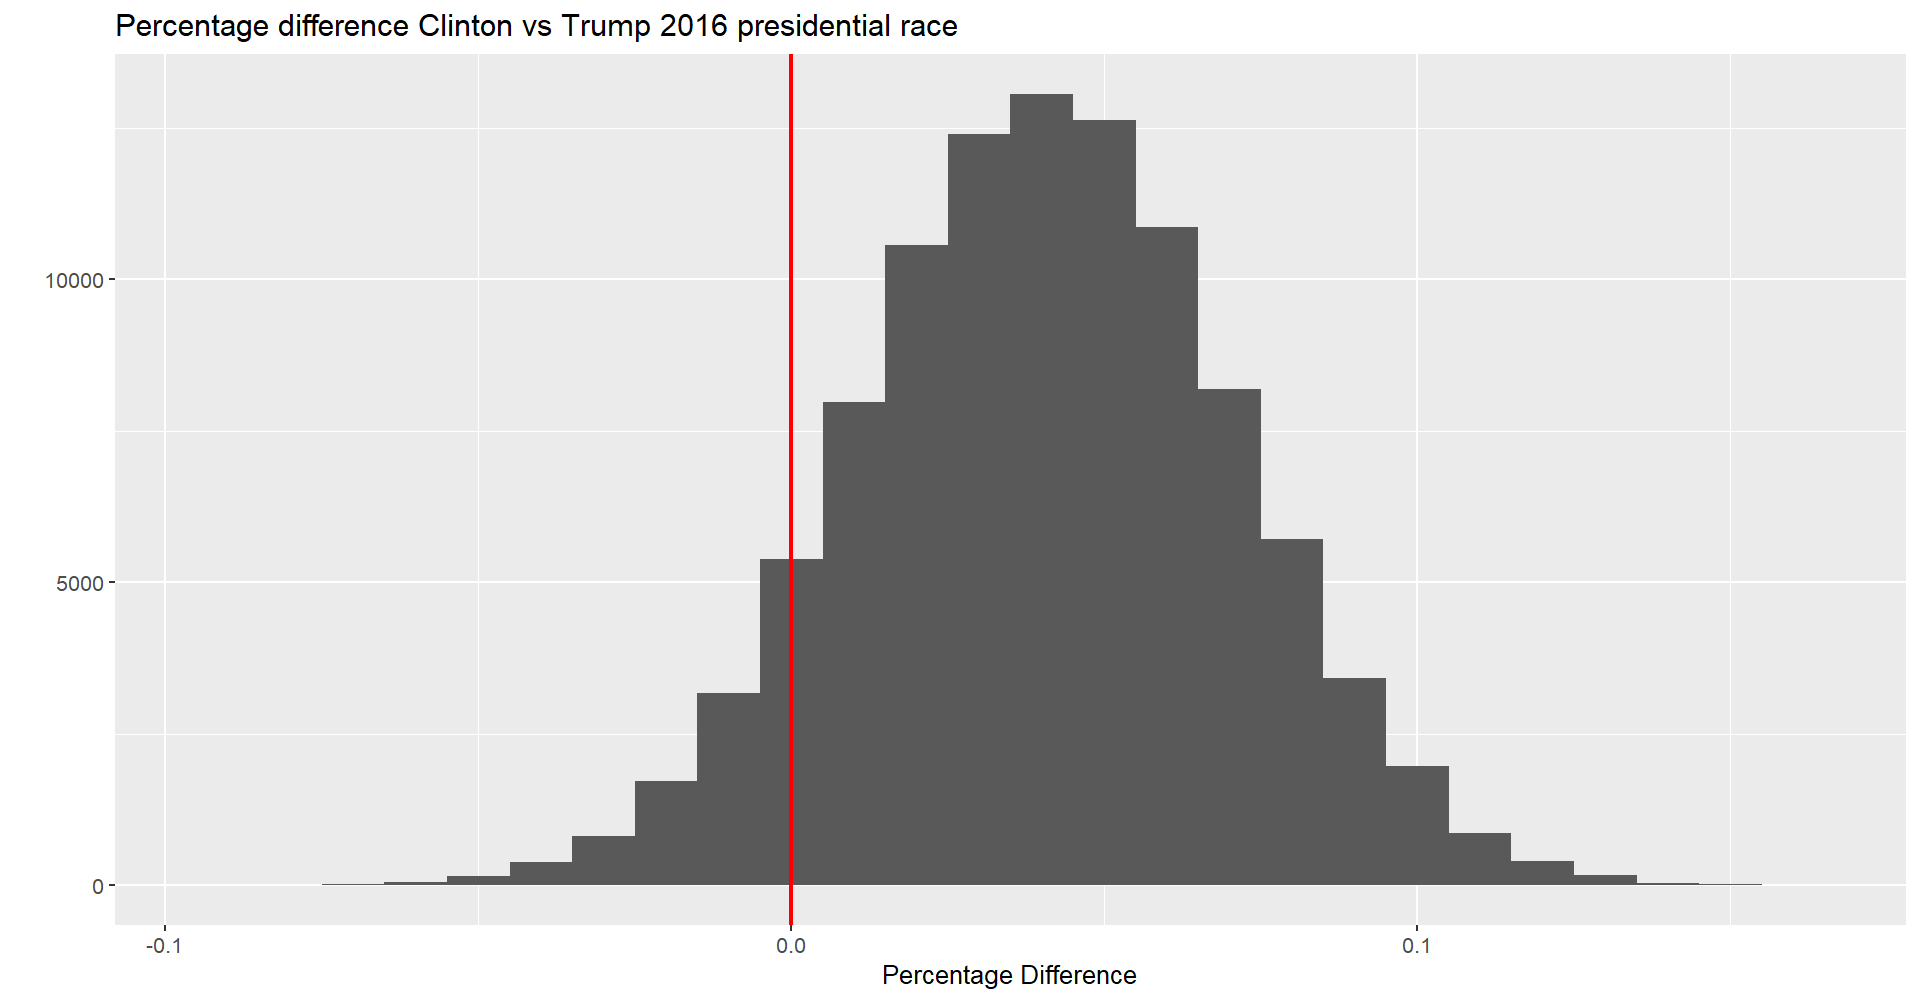
\includegraphics[width=340pt, height=200pt]{Chapters/chapter4/figures/hiillaryVStrump.png}
	%%\centerline{\epsfig{/Chapters/chapter1/figures/cat.eps,width=.8\textheight,height=.4\textwidth}}
	\caption[List of figure caption goes here]{Percentage difference: Hillary Clinton vs Donald Trump, five-way race.}\label{fig41}
\end{figure}

There is a 95\% probability that the percentage difference between Hillary and Trump according to this poll is (-1.8\%, 9.9\%). The probability of Hillary having more supporters is 91.3\%


\begin{tcolorbox}[enhanced,width=4.67in,center upper,
	fontupper=\large\bfseries,drop shadow southwest,sharp corners]
	\textit{R code. Multinomial-Dirichlet mdoel: Liverpool vs Manchester city}
\begin{VF}
\begin{lstlisting}[basicstyle=\footnotesize, language=R]
2. Quantiles for each variable:

2.5%      25%      50%      75%    97.5% 
-0.01817  0.02033  0.04058  0.06089  0.09923 
CW <- mean(difmcmc>0)
CW
0.91339

# Predictive distribution by simulation
y0 <- c(44, 40, 16)

Pred <- apply(thetas, 1, function(p) {
	rmultinom(1, size = sum(y0), prob = p)})
sum(sapply(1:S, function(s) {
	sum(Pred[,s] == y0) == 3}))/S
0.00825

# Predictive distribution by analytical expression
PredY0 <- function(y0){
	n <- sum(y0)
	Res1 <- sum(sapply(1:length(y), function(l){
		lgamma(alphan[l]+y0[l]) - 
		lgamma(alphan[l])-lfactorial(y0[l])}))
	Res <- lfactorial(n)+lgamma(sum(alphan))
	-lgamma(sum(alphan)+n) + Res1
	return(exp(Res))
}
PredY0(y0)
0.00850         
\end{lstlisting}
\end{VF}
\end{tcolorbox} 

The probability that from one hundred random selected people 44 support Hillary, 40 support Trump and 16 support other candidate is 0.85\%.

\item \textbf{Math test example continues}

You have a random sample of math scores of size $N=50$ from a normal distribution, $Y_i\sim \mathcal{N}(\mu, \sigma)$. The sample mean and variance are equal to $102$ and $10$, respectively. Using the normal-normal/inverse-gamma model where $\mu_0=100$, $\beta_0=1$, $\alpha_0=\delta_0=0.001$

\begin{itemize}
	\item Get a 95\% confidence and credible interval for $\mu$.
	\item What is the posterior probability that $\mu > 103$?  
\end{itemize}  

{\textbf{Answer}}

\begin{tcolorbox}[enhanced,width=4.67in,center upper,
	fontupper=\large\bfseries,drop shadow southwest,sharp corners]
	\textit{R code. Math test example continues}
\begin{VF}
\begin{lstlisting}[basicstyle=\footnotesize, language=R]
set.seed(010101)
N <- 50
# Sample size
muhat <- 102
# Sample mean
sig2hat <- 10
# Sample variance

# Hyperparameters
mu0 <- 100
beta0 <- 1
delta0 <- 0.001
alpha0 <- 0.001

S <- 100000
# Posterior draws
alphan <- alpha0 + N
deltan <- sig2hat*(N - 1) + delta0 + 
beta0*N/(beta0 + N)*(muhat - mu0)^2
sig2Post <- invgamma::rinvgamma(S, shape = alphan, 
rate = deltan)
summary(sig2Post)
betan <- beta0 + N
mun <- (beta0*mu0 + N*muhat)/betan
muPost <- sapply(sig2Post, function(s2){rnorm(1, mun, 
	sd = (s2/betan)^0.5)})

muPostq <- quantile(muPost, c(0.025, 0.5, 0.975))
muPostq
   2.5%      50%    97.5% 
101.0929 101.9625 102.8311
cutoff <- 103
PmuPostcutoff <- mean(muPost > cutoff)
PmuPostcutoff
0.00994
# Using Student's t
muPost_t <- ((deltan/(alphan*betan))^0.5)*rt(S, alphan)
 + mun
c1 <- rgb(173,216,230,max = 255, alpha = 50, 
names = "lt.blue")
c2 <- rgb(255,192,203, max = 255, alpha = 50, 
names = "lt.pink")
hist(muPost, main = "Histogram: Posterior mean", 
xlab = "Posterior mean", col = c2)
hist(muPost_t, main = "Histogram: Posterior mean", 
xlab = "Posterior mean", add = T, col = c1)
muPost_tq <- quantile(muPost_t, c(0.025, 0.5, 0.975))
muPost_tq
2.5%      50%    97.5% 
101.0837 101.9608 102.8435
PmuPost_tcutoff <- mean(muPost_t > cutoff)
PmuPost_tcutoff
0.01087
\end{lstlisting}
\end{VF}
\end{tcolorbox} 

We perform our calculations using the posterior conditional distribution, and the posterior marginal distribution. Both procedures give similar results as we can observe from Figure \ref{fig42}.

\begin{figure}[!h]
	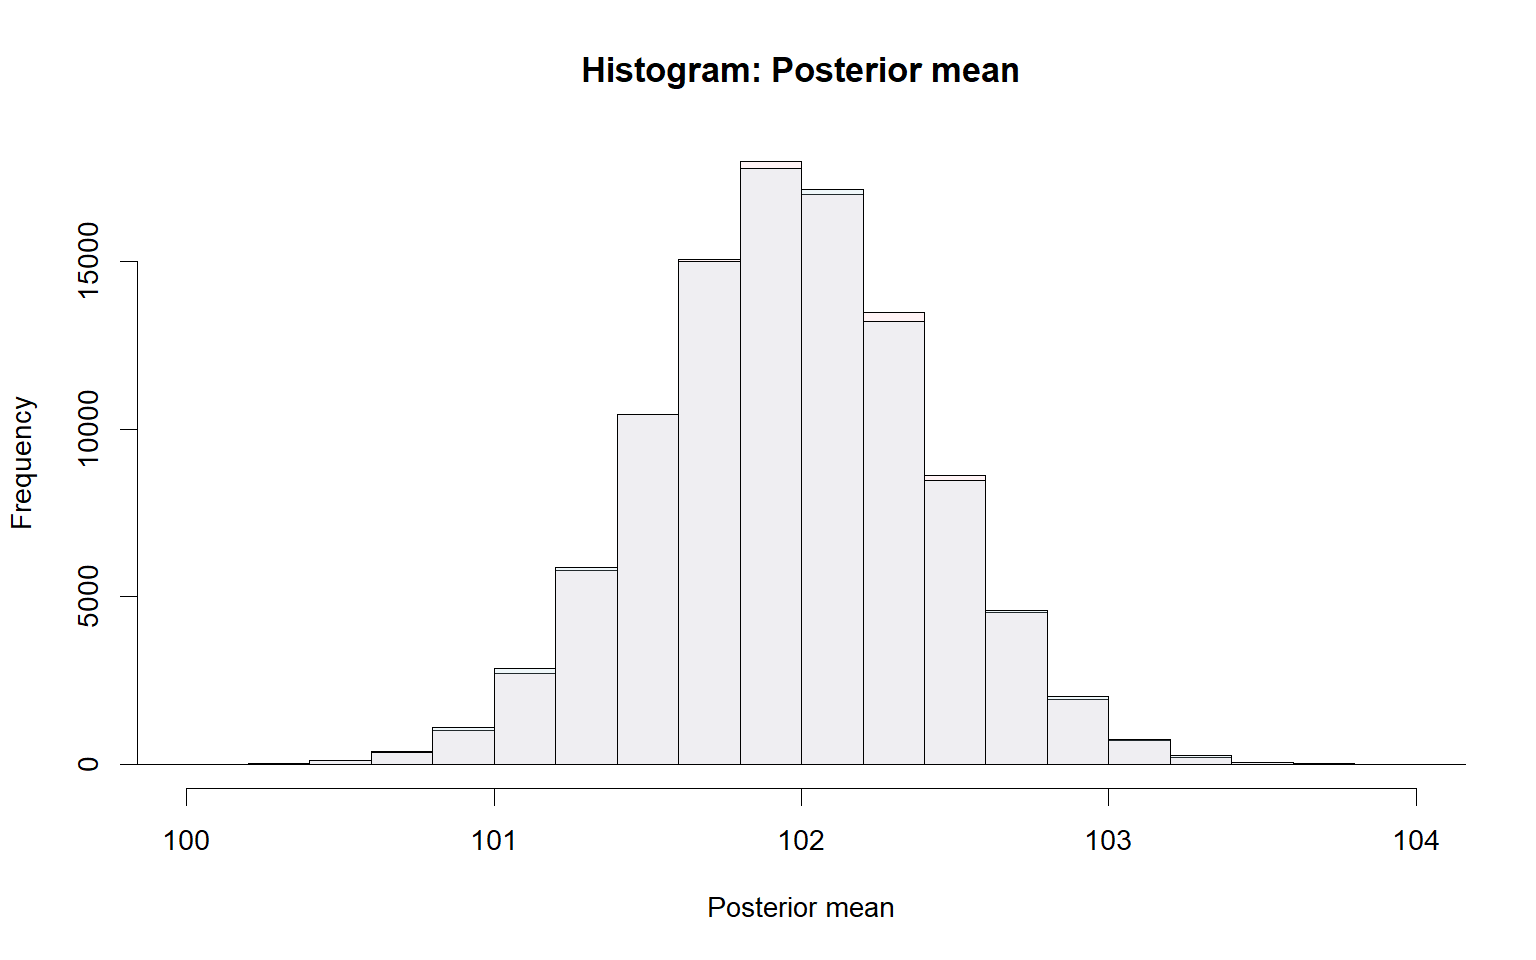
\includegraphics[width=340pt, height=200pt]{Chapters/chapter4/figures/conditionalVSmarginal.png}
	%%\centerline{\epsfig{/Chapters/chapter1/figures/cat.eps,width=.8\textheight,height=.4\textwidth}}
	\caption[List of figure caption goes here]{Histogram using the posterior conditional distribution and the posterior marginal distribution}\label{fig42}
\end{figure}


We have that the 95\% credible interval is (101.08, 102.84), and the probability of having a value greater than 103 is 1.09\%. 


 

\item In the optimal tangency portfolio example, what are the equations for $\mu_{T+\kappa}=\mu_{n}$ and ${\bf\Sigma}_{T+\kappa}$? Use these equations to find the optimal weights six periods ahead using the tech stocks. 

{\textbf{Answer}}  


\end{enumerate}



